%%% Please, do not change any of the following parameters.
\documentclass[10pt,journal,compsoc,twoside]{IEEEtran}
\usepackage{cite}
\usepackage{graphicx}
\usepackage{amsmath}
%\interdisplaylinepenalty=2500
\usepackage{algorithmic}
\usepackage{array}
\usepackage[caption=false,font=footnotesize]{subfig}
\usepackage{url}
\usepackage{lipsum}
\usepackage{hyperref}
\hypersetup{pdfborder = 0 0 0}
\PassOptionsToPackage{hyphens}{url}\usepackage{hyperref}
\newcommand{\Ref}[2]{#2 \ref{#1}}
\newcommand{\fromto}[5]{(#1 #3 $<$ #4 $<$ #2 #3)}
\graphicspath{ {figures/} } %%% put all images file into "figures/" subdirectory
\usepackage[detect-all]{siunitx}
\newcommand{\me}{\mathrm{e}}

\begin{document}

\title{Emotion recognition in computer games and films}

\author{Filip Rynkiewicz%
\IEEEcompsocitemizethanks{\IEEEcompsocthanksitem Lodz University of Technology, Lodz, Poland, \hfil\break 	filip.rynkiewicz@dokt.p.lodz.pl}}


% The paper headers
\markboth{Computer Game Innovations, 2017}%
{}

\IEEEtitleabstractindextext{%
\begin{abstract}
%%% 100 words
In last years technology used in game and film creations has formed a need to check people's reaction to watched images. Human body reacts on external stimulus by face microchanges, distortions in electroencephalography, pupil adjustments etc. Those processes can be recorded with specific apparatus thus correct analysis of those characteristics can be automated. Thanks to this authors are able to check viewer's to their creations, or even construct algorithms that can do it automatically.

\end{abstract}

\begin{IEEEkeywords}
 emotion recognition, pupil reflex, EEG, electroencephalography, emotion clasificcation
\end{IEEEkeywords}}

\maketitle
\IEEEdisplaynontitleabstractindextext
\IEEEpeerreviewmaketitle
\IEEEraisesectionheading{
\section{Introduction}
}
Studies on recognition of the human emotions can be useful in many areas. Starting with psychology studies on behavioural disorder with patient that have problems with expressing emotions, through biology studies on creation of emotions in human body and ending with getting feedback from a watched movie. Emotions allow to decide if users like what they see or not. That gives them an opportunity to choose if they wants to end it immediately, or even repeat these emotions again. For artists this informations is very desirable, because they can refine their creations based on the information gathered from user's reactions. Thanks to such research artist will know when users will be more interested in action, when it will be more dull or touching for them. 

In \cite{OrtonyCloreCollins1988} authors created a theory which explains generation of emotions in human body. They simplify it to few steps, like in a algorithm. First there is a perception of an event then analysis of it based on user's own experience and norms, so finally the event can be classified as certain emotion.

Emotions can be detected by certain characteristics that could be classified as one of the two groups:
\begin{itemize}
	\item psychological:
	\begin{itemize}
		\item EEG(electroencephalography),
		\item EMG(electromyography), 
		\item EKG(electrocardiography), 
		\item pupil diameter.
	\end{itemize} 
	\item non-psychological: 
	\begin{itemize} 
		\item text, 
		\item speech,
		\item  gestures, 
		\item facial expressions.
	\end{itemize}
\end{itemize}
This paper will focus on group of psychological signals, especially on EEG and pupil diameter. It will be explained how to detect certain emotion based on fusions of the stimuli. There are plenty of researches where authors combine EEG with pupil diameter or even with eye trackers data, and those combined methods are more reliable and have better accuracy then individual ones \cite{WeiLongBoNanBaoLiang2014,CalvoDMello2010,SoleymaniPanticPun2002}. 

\subsection{Subjects and stimuli}
Using a variety of movie clips, especially selected for this research and shown to participators, the EEG signal and pupil diameter changes were recorded. The key feature of those movie clips is to cover different emotional responses to get the best and as accurate results. Psychologists recommended videos from 1 to 10 minutes long for elicitation of single emotion\cite{SchaeferNilsSanchezPhilippot2010}.

\section{EEG}
The most popular methods of emotion recognition are based on analysis of electroencephalography signals. Numerous researches\cite{LinMusic,GaoMehmood,NieWangShiLu,AdolphsTranesDamasio2003,DamasioGrabowski2000} has shown that the brain activity, which EEG collects, is the most reliable source for emotion recognition. The core of those studies is to find brain regions and frequency bands most related to those emotions. Studies of \cite{SarloBuodoPoliPalomba} showed that activation for unpleasant emotions was prominent over the right posterior regions in the alpha band. In \cite{SchmidtTrainor2001} authors found that frontal brain electrical activity is closely related to musical emotions, and in \cite{LiLu2009} authors confirmed a theory that gamma band is also related to music emotions.

\subsection{Data acquisition} 
Gathering data of brain activity is done by using special EEG cap, where \textit{AgCl} electrodes placed on it are collecting brain activity in certain areas. Most commonly used layout of electrodes is 10-20 system, shown in \Ref{fig:1020electrodes}{Figure}.

\begin{figure}[ht]
	\centering
	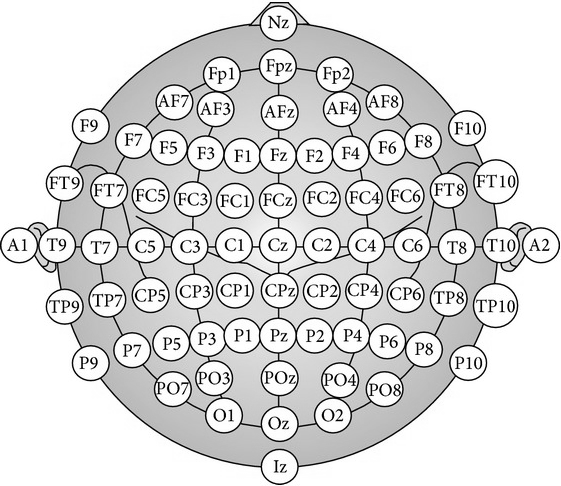
\includegraphics[width=0.7\linewidth]{10_20_electrodes}
	\caption{The EEG cap arrangement for 10-20 system.\cite{JirayucharoensakSuwichaPanngumIsrasenaPasin2014}}
	\label{fig:1020electrodes}
\end{figure}

Signals were recorded mostly in \numrange[range-phrase = --]{1000}{1024} Hz sampling rate. To speed up calculations those characteristics were down sampled to \numrange[range-phrase = --]{200}{256} Hz. Noises and artefacts reduction were done by applying bypass filter between  \numrange{0.5}{70} Hz.
\subsection{Data extraction}
Correlation of certain spectral power of EEG signal and emotions relevant processing was observed \cite{AftanasSavotinaMakhnev2005}. There are multiple methods of extracting power spectral density (PSD) from raw signals. Two of them will be expounded.

First \cite{WeiLongBoNanBaoLiang2014} use Fourier transform and Welch algorithm. This method splits signal into overlapping segments and the PSD is estimated by averaging the periodograms. In result the power spectrum is smoother. PSD of individual electrodes was estimated using 15s long windows with 50 percent overlapping. PSD bands like theta \fromto{4}{8}{Hz}{f} \  ,  slow alpha \fromto{6}{10}{Hz}{f} \  ,  alpha \fromto{8}{12}{Hz}{f} \  ,  beta \fromto{12}{30}{Hz}{f} \\  and  gamma 30Hz $<$ f were extracted from electrodes. In additional 14 symmetrical pairs on the right and left hemisphere were extracted to measure possible asymmetry in brain activity.
\newline
\newline
Second one use a short-time Fourier transform with non-overlapped Hanning window of 4 s. In addition to PSD the differential entropy (DE), differential asymmetry (DASM) and rational asymmetry (RASM) were extracted and compared. Like in first method five frequency bands were used. Delta \fromto{1}{3}{Hz}{f} \  ,  theta \fromto{4}{7}{Hz}{f} \  ,  alpha \fromto{8}{13}{Hz}{f} \  ,  beta \fromto{14}{30}{Hz}{f} \\ and  gamma \fromto{31}{50}{Hz}{f} \,. Using \Ref{eq:DE}{equation}, DE was calculated.
\begin{equation}
\begin{aligned}
h(X)=\int\limits_{-\infty}^{\infty} \frac{1}{\sqrt{2\pi\sigma^{2}}}exp \frac{(x - \mu)^{2}}{2\sigma^{2}}log\frac{1}{\sqrt{2\pi\sigma^{2}}}\\ exp\frac{(x - \mu)^{2}}{2\sigma^{2}}dx = \frac{1}{2}log2\pi \me \sigma^{2}
\end{aligned}
\label{eq:DE}
\end{equation}
where X is Gauss distribution $N(\mu, \sigma^2)$, \textit{x} is a variable $\pi$ and $\me$ are constants. DASM and RASM are defined as :
\begin{equation}
DASM = h(X_{LEFT}) - h(X_{RIGHT})
\end{equation}
\begin{equation}
RASM = h(X_{LEFT}) / h(X_{RIGHT})
\end{equation}
where $X_{LEFT}$ and$X_{RIGHT}$ are DE features of left and right hemisphere of brain.
\newpage
\subsection{Classification}
After the data was collected and extracted the support vector machine (SVM) was used as classifier, in both examples.
In  \cite{WeiLongBoNanBaoLiang2014} they smoothed features using linear dynamic system (LDS).

\begin{figure}[ht]
	\centering
	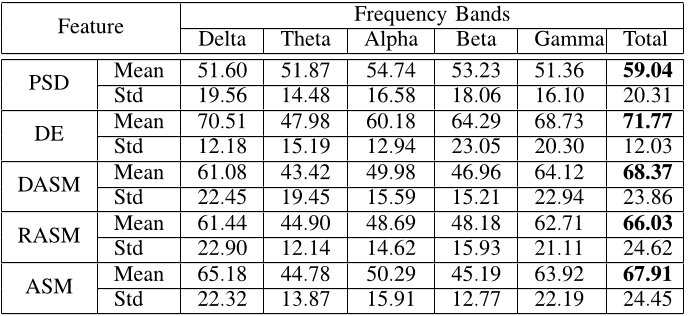
\includegraphics[width=1.0\linewidth]{performanceOfClassifier1}
	\caption{The performance of classifiers in \% using different kinds of frequency band features. For \cite{WeiLongBoNanBaoLiang2014}.}
	\label{fig:performanceofclassifier1}
\end{figure}
Result of classification can be bee seen at \Ref{fig:performanceofclassifier1}{Figure}. ASM feature is concatenation of DASM nad RASM. As we can see, delta and gamma frequency bands perform better than theta and alpha frequency bands, and total frequency band has a stable and  prominent  accuracy.  Also  we  can  see  that,  differential entropy features get best accuracies in almost all frequency  bands  except  Theta  band  (47.98\%  of  DE  features is  less  than  51.87\%  of  PSD  features).
\newline
\par In \cite{SoleymaniPanticPun2002} in EEG there was only DE feature. They have used SVM classification with RBF kernel.
\begin{figure}[ht]
	\centering
	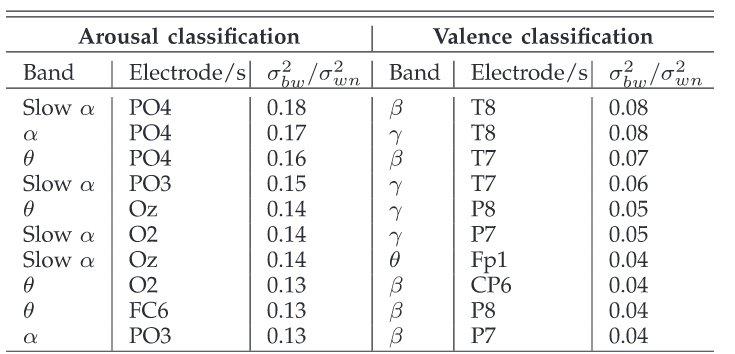
\includegraphics[width=1.0\linewidth]{performanceOfClassifier2}
	\caption{The performance of classifiers using different kinds of frequency band features. For \cite{SoleymaniPanticPun2002}.}
	\label{fig:performanceofclassifier2}
\end{figure}
The linear discrimination criterion was calculated for EEG signals. Dividing between class variance by within class variance for any given feature.
For arousal classification, PSD in alpha bands of occipital electrodes was found to have the most discriminant features. In contrast, valence beta and gamma bands of temporal electrodes are more informative. The between class to within class variance ratios are higher for the best arousal EEG features. The higher linear discrimination criterion for best arousal features explains the superior classification rate for arousal dimension.



\section{Pupil diameter}
The theory was forged based on the observation of the human eye. Pupil diameter is changing in different emotional states. The disadvantage of this solution is that pupil's diameter is highly dependant on the light. First step to gathering data from a pupil is to create lighting reflex model. The most common and the simplest method is principal component analysis (PCA).
\subsection{Light reflex model}
Assuming that \textit{Y} is the $M \times N_{p}$ matrix of pupillary response for the same picture for \textit{$N_{p}$} participant and \textit{M} samples, \textit{Y} consists of three components
\begin{equation}
Y = A + B + C
\end{equation}
where \textit{A} is the lighting influence, \textit{B} is the emotional response and \textit{C} is the noise. Extracting first component from PCA to approximate the pupil response for the lightning changes during the experiments.
\subsection{Data acquisition}
To gather the data the Eye-Tracker devices were used. These apparatus are able to collect position of the projected eye gaze on the screen, pupil diameter, moments when the eyes were closed and a distance of the participant's eyes to the gaze tracker device. Eye blinking creates gaps in eye gaze and pupil record, thus the linear interpolation was used to replace missing samples.
\begin{figure}[ht]
	\centering
	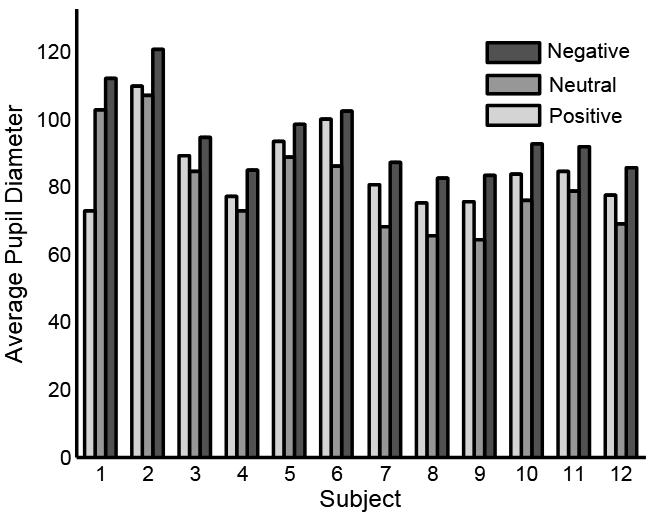
\includegraphics[width=1.0\linewidth]{pupilDiameter1}
	\caption{Average pupil diameter. For \cite{WeiLongBoNanBaoLiang2014}.}
	\label{fig:pupilSize1}
\end{figure}
\newline
As it can be seen at \Ref{fig:pupilSize1}{Figure} for 12 participants the smallest average value have neutral emotion, except subject 1.

\begin{figure}[ht]
	\centering
	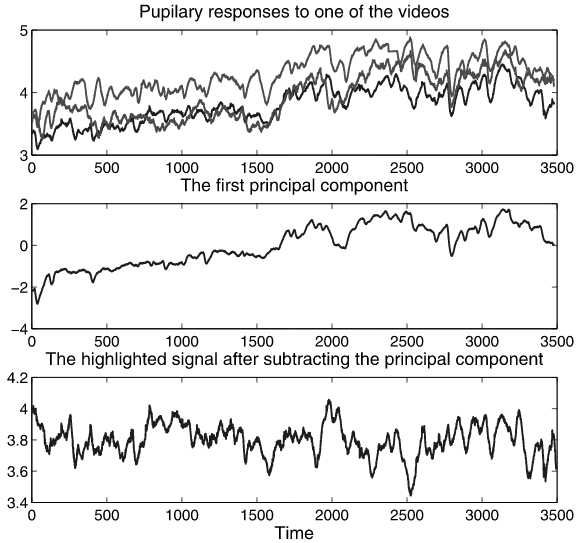
\includegraphics[width=1.0\linewidth]{pupilDiameter2}
	\caption{
		From top to bottom: In the first plot, there is an example of pupil diameter measures from three different participants in response to one video. The second plot shows the first principal component extracted by PCA from the time series shown in the first plot (the lighting effect). The bottom plot shows the pupil diameter of the blue signal in the first plot after reducing the lighting effect\cite{SoleymaniPanticPun2002}}
	\label{fig:pupilDiameter2}
\end{figure}

At \Ref{fig:pupilDiameter2}{Figure} the examples of pupillary responses, extracted pupillary lighting reflex, and the residual component after removing the light reflex are given.
\subsection{Classification}
As in the EEG for classification of signal, for both examples, the SVM was used.
\begin{figure}[ht]
	\centering
	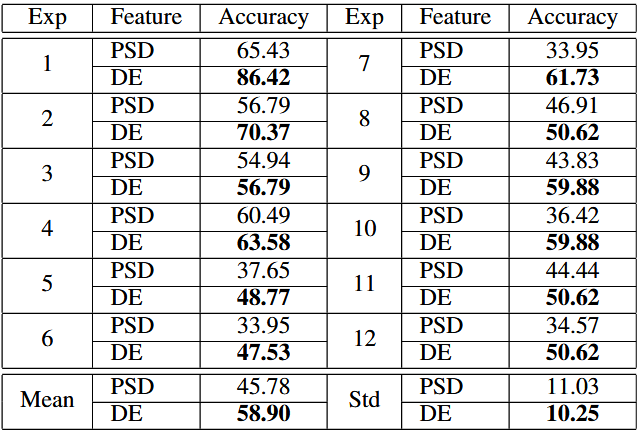
\includegraphics[width=1.0\linewidth]{performanceOfClassifierPupil1}
	\caption{ Performence in \% of using different features from pupil diameter \cite{WeiLongBoNanBaoLiang2014}}
	\label{fig:performanceOfClassifierPupil1}
\end{figure}
As it can be seen at \Ref{fig:performanceOfClassifierPupil1}{Figure} the DE feature performs much better than PSD, because DE features have the balance ability of discriminating patterns between  lowand high frequency energy.
 \section{Multimodial Fusion} 
After the data was gathered the fusion of methods is what's left. Examples used in this article have implemented the feature level fusion and decision level fusion. 
\subsection{Feature level fusion}
In this approach the features vectors from different stimuli were concatenated to form larger feature vector.
\subsection{Decision level fusion}
Two classifiers were trained with different features, and were fused to generate a new classification using some new principles or learning algorithms. In \cite{WeiLongBoNanBaoLiang2014} they applied two principles. One was called max strategy which selected the higher probabilistic outputs of classifiers trained with a single modality separately as final result. Another was called sum strategy which summed up probabilities of same emotions from different frequency bands and selected the highest one.
\subsection{Results}
Overall results of experiments for \cite{WeiLongBoNanBaoLiang2014} are shown at \Ref{fig:result1}{Figure}.
We see that decision level fusion using max strategy and feature level fusion performed better than single modality like EEG or pupil diameter, which achieved average accuracies of 72.98\% and 73.59\%, respectively.
\begin{figure}[ht]
	\centering
	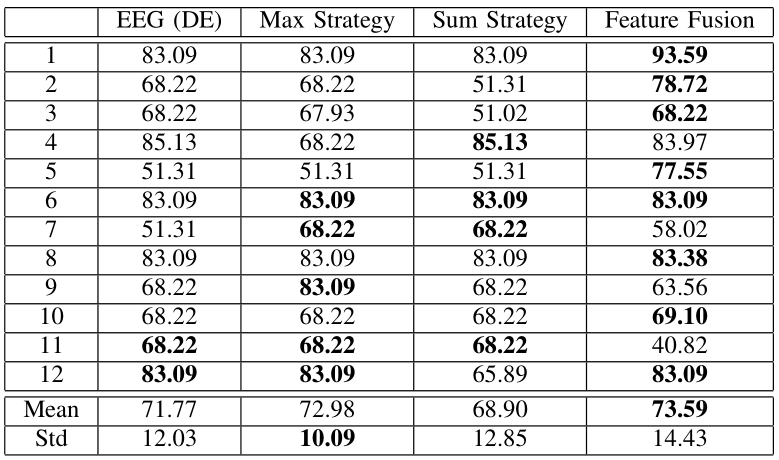
\includegraphics[width=1.0\linewidth]{result1}
	\caption{ Performance in \% of using different multimodal features \cite{WeiLongBoNanBaoLiang2014}}
	\label{fig:result1}
\end{figure}

Another results \Ref{fig:result2}{Figure} for \cite{SoleymaniPanticPun2002} has shown that the DLF have the best accuracy for arousal and valance. 

\begin{figure}[ht]
	\centering
	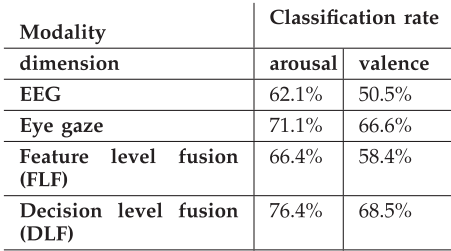
\includegraphics[width=0.7\linewidth]{result2}
	\caption{ Performance in \% of using different multimodal features \cite{SoleymaniPanticPun2002}}
	\label{fig:result2}
\end{figure}

Difference of results of both researches are really high. For FLF the percentage is  accordingly 66.4 \% and 73.59\%. EEG for PSD feature 62.1 \% and 71.77\% for DE feature.
\section{Conclusion}

Emotions are sophisticated mechanism in human body, but knowledge how they work can be helpful in many areas. Those signals can be obtained from many of human impulses, such as pupil reflex or brain signals. Using appropriate techniques and devices those characteristics can be collected and analysed to detect emotions. Combining those modalities and fusing it with special techniques can lead to better accuracy of methods.
	




\begin{thebibliography}{99}
\bibitem{OrtonyCloreCollins1988}A. Ortony, G.L. Clore, A. Collins \textit{The Cognitive Structure of Emotions.}, Cambridge University Press, July 1988.
\bibitem{CalvoDMello2010} R. A. Calvo, S.D'Mello \textit{Affect detection: An interdisciplinary review of models, methods and their applications}, IEEEE Transactions on Affective Computing, vol 1, no1, pp 18-37, 2010
\bibitem{SoleymaniPanticPun2002} M. Soleymani, M. Pantic, T. Pun \textit{Multimodal Emotion Recognition in Responce to Videos}, IEEE Transaction on Affective Computing, vol. 3, no. 2, april-June 2012
\bibitem{AdolphsTranesDamasio2003}R. Adolphs, D. Tranel, A.R. Damasio, \textit{Dissociable Neural Systems for Recognizing Emotions}, Brain and Cognition, vol. 52, no. 1, pp. 61-69, June 2003.
\bibitem{DamasioGrabowski2000} A.R. Damasio, T.J. Grabowski, A. Bechara, H. Damasio, L.L.B. Ponto, J. Parvizi, and R.D. Hichwa, \textit{Subcortical and Cortical Brain
Activity during the Feeling of Self-Generated Emotions}, Nature
Neuroscience, vol. 3, no. 10, pp. 1049-1056, Oct. 2000.
\bibitem{WeiLongBoNanBaoLiang2014} Z. Wei-Long, D. Bo-Nan , L. Bao-Liang 
\textit{Multimodal Emotion Recognition using EEG and Eye Tracking Data}, IEEE, 2014
\bibitem{LinMusic}
Y. P. Lin, \textit{EEG-Based Emotion Recognition in Music Listening},IEEE Transactions on Biomedical Engineering, vol. 57, no. 7, pp. 1798-1806, July 2010.
\url{http://ieeexplore.ieee.org/stamp/stamp.jsp?tp=&arnumber=5458075&isnumber=5484937}
\bibitem{GaoMehmood}
Y. Gao, H. J. Lee and R. M. Mehmood, \textit{Deep learninig of EEG signals for emotion recognition}, IEEE, International Conference on Multimedia \& Expo Workshops (ICMEW), Turin, 2015, pp. 1-5.
\url{http://ieeexplore.ieee.org/stamp/stamp.jsp?tp=&arnumber=7169796&isnumber=7169738}
\bibitem{NieWangShiLu}Dan Nie, Xiao-Wei Wang, Li-Chen Shi, and Bao-Liang Lu, \textit{EEG-based Emotion Recognition during Watching Movies}, IEEE, Proceedings of the 5th International IEEE EMBS Conference on Neural Engineering Cancun, Mexico, April 27 - May 1, 2011 ,\url{https://pdfs.semanticscholar.org/6511/590bc9677922c82747b5d183383f46b50db6.pdf}

\bibitem{SarloBuodoPoliPalomba}
 M. Sarlo, G. Buodo, S. Poli, and D. Palomba, \textit{Changes in EEG alpha
power to different disgust elicitors: the specificity of mutilations}
Neuroscience Letters, vol. 382, no.3, pp. 291-296, 2005.
\bibitem{SchmidtTrainor2001}
 L. A. Schmidt, and L. J. Trainor, \textit{Frontal brain electrical activity
distinguishes valence and intensity of musical emotions} Cognition
and Emotion, vol. 15, no. 4, pp. 487-500, 2001.
\bibitem{LiLu2009}
M. Li, and B. L. Lu, \textit{Emotion classification based on gamma-band
EEG} IEEE Int. Conf. Engineering in Medicine and Biology Society,
Minneapolis, 2009, pp. 1223-1226.
\bibitem{JirayucharoensakSuwichaPanngumIsrasenaPasin2014}
Jirayucharoensak, Suwicha  Pan-ngum, Setha  Israsena, Pasin. \textit{EEG-Based Emotion Recognition Using Deep Learning Network with Principal Component Based Covariate Shift Adaptation}, TheScientificWorldJournal. 2014. 
 \bibitem{SchaeferNilsSanchezPhilippot2010}
A.Schaefer ,F. Nils  and  X. Sanchez  and  P. Philippot,
\textit{Assessing the effectiveness of a large database of emotion-eliciting films: A new tool for emotion researchers}, 2010
\bibitem{AftanasSavotinaMakhnev2005}
Aftanas, L.I., Savotina, L.N., Makhnev, V.P. et al.\textit{ Neurosci Behav Physiol}, 2005

\end{thebibliography}



\end{document}


